% Options for packages loaded elsewhere
\PassOptionsToPackage{unicode}{hyperref}
\PassOptionsToPackage{hyphens}{url}
\PassOptionsToPackage{dvipsnames,svgnames*,x11names*}{xcolor}
%
\documentclass[
]{article}
\usepackage{lmodern}
\usepackage{amsmath}
\usepackage{ifxetex,ifluatex}
\ifnum 0\ifxetex 1\fi\ifluatex 1\fi=0 % if pdftex
  \usepackage[T1]{fontenc}
  \usepackage[utf8]{inputenc}
  \usepackage{textcomp} % provide euro and other symbols
  \usepackage{amssymb}
\else % if luatex or xetex
  \usepackage{unicode-math}
  \defaultfontfeatures{Scale=MatchLowercase}
  \defaultfontfeatures[\rmfamily]{Ligatures=TeX,Scale=1}
\fi
% Use upquote if available, for straight quotes in verbatim environments
\IfFileExists{upquote.sty}{\usepackage{upquote}}{}
\IfFileExists{microtype.sty}{% use microtype if available
  \usepackage[]{microtype}
  \UseMicrotypeSet[protrusion]{basicmath} % disable protrusion for tt fonts
}{}
\makeatletter
\@ifundefined{KOMAClassName}{% if non-KOMA class
  \IfFileExists{parskip.sty}{%
    \usepackage{parskip}
  }{% else
    \setlength{\parindent}{0pt}
    \setlength{\parskip}{6pt plus 2pt minus 1pt}}
}{% if KOMA class
  \KOMAoptions{parskip=half}}
\makeatother
\usepackage{xcolor}
\IfFileExists{xurl.sty}{\usepackage{xurl}}{} % add URL line breaks if available
\IfFileExists{bookmark.sty}{\usepackage{bookmark}}{\usepackage{hyperref}}
\hypersetup{
  pdftitle={Supplementary Information},
  colorlinks=true,
  linkcolor=Maroon,
  filecolor=Maroon,
  citecolor=Blue,
  urlcolor=blue,
  pdfcreator={LaTeX via pandoc}}
\urlstyle{same} % disable monospaced font for URLs
\usepackage[margin=1in]{geometry}
\usepackage{color}
\usepackage{fancyvrb}
\newcommand{\VerbBar}{|}
\newcommand{\VERB}{\Verb[commandchars=\\\{\}]}
\DefineVerbatimEnvironment{Highlighting}{Verbatim}{commandchars=\\\{\}}
% Add ',fontsize=\small' for more characters per line
\usepackage{framed}
\definecolor{shadecolor}{RGB}{248,248,248}
\newenvironment{Shaded}{\begin{snugshade}}{\end{snugshade}}
\newcommand{\AlertTok}[1]{\textcolor[rgb]{0.94,0.16,0.16}{#1}}
\newcommand{\AnnotationTok}[1]{\textcolor[rgb]{0.56,0.35,0.01}{\textbf{\textit{#1}}}}
\newcommand{\AttributeTok}[1]{\textcolor[rgb]{0.77,0.63,0.00}{#1}}
\newcommand{\BaseNTok}[1]{\textcolor[rgb]{0.00,0.00,0.81}{#1}}
\newcommand{\BuiltInTok}[1]{#1}
\newcommand{\CharTok}[1]{\textcolor[rgb]{0.31,0.60,0.02}{#1}}
\newcommand{\CommentTok}[1]{\textcolor[rgb]{0.56,0.35,0.01}{\textit{#1}}}
\newcommand{\CommentVarTok}[1]{\textcolor[rgb]{0.56,0.35,0.01}{\textbf{\textit{#1}}}}
\newcommand{\ConstantTok}[1]{\textcolor[rgb]{0.00,0.00,0.00}{#1}}
\newcommand{\ControlFlowTok}[1]{\textcolor[rgb]{0.13,0.29,0.53}{\textbf{#1}}}
\newcommand{\DataTypeTok}[1]{\textcolor[rgb]{0.13,0.29,0.53}{#1}}
\newcommand{\DecValTok}[1]{\textcolor[rgb]{0.00,0.00,0.81}{#1}}
\newcommand{\DocumentationTok}[1]{\textcolor[rgb]{0.56,0.35,0.01}{\textbf{\textit{#1}}}}
\newcommand{\ErrorTok}[1]{\textcolor[rgb]{0.64,0.00,0.00}{\textbf{#1}}}
\newcommand{\ExtensionTok}[1]{#1}
\newcommand{\FloatTok}[1]{\textcolor[rgb]{0.00,0.00,0.81}{#1}}
\newcommand{\FunctionTok}[1]{\textcolor[rgb]{0.00,0.00,0.00}{#1}}
\newcommand{\ImportTok}[1]{#1}
\newcommand{\InformationTok}[1]{\textcolor[rgb]{0.56,0.35,0.01}{\textbf{\textit{#1}}}}
\newcommand{\KeywordTok}[1]{\textcolor[rgb]{0.13,0.29,0.53}{\textbf{#1}}}
\newcommand{\NormalTok}[1]{#1}
\newcommand{\OperatorTok}[1]{\textcolor[rgb]{0.81,0.36,0.00}{\textbf{#1}}}
\newcommand{\OtherTok}[1]{\textcolor[rgb]{0.56,0.35,0.01}{#1}}
\newcommand{\PreprocessorTok}[1]{\textcolor[rgb]{0.56,0.35,0.01}{\textit{#1}}}
\newcommand{\RegionMarkerTok}[1]{#1}
\newcommand{\SpecialCharTok}[1]{\textcolor[rgb]{0.00,0.00,0.00}{#1}}
\newcommand{\SpecialStringTok}[1]{\textcolor[rgb]{0.31,0.60,0.02}{#1}}
\newcommand{\StringTok}[1]{\textcolor[rgb]{0.31,0.60,0.02}{#1}}
\newcommand{\VariableTok}[1]{\textcolor[rgb]{0.00,0.00,0.00}{#1}}
\newcommand{\VerbatimStringTok}[1]{\textcolor[rgb]{0.31,0.60,0.02}{#1}}
\newcommand{\WarningTok}[1]{\textcolor[rgb]{0.56,0.35,0.01}{\textbf{\textit{#1}}}}
\usepackage{graphicx}
\makeatletter
\def\maxwidth{\ifdim\Gin@nat@width>\linewidth\linewidth\else\Gin@nat@width\fi}
\def\maxheight{\ifdim\Gin@nat@height>\textheight\textheight\else\Gin@nat@height\fi}
\makeatother
% Scale images if necessary, so that they will not overflow the page
% margins by default, and it is still possible to overwrite the defaults
% using explicit options in \includegraphics[width, height, ...]{}
\setkeys{Gin}{width=\maxwidth,height=\maxheight,keepaspectratio}
% Set default figure placement to htbp
\makeatletter
\def\fps@figure{htbp}
\makeatother
\setlength{\emergencystretch}{3em} % prevent overfull lines
\providecommand{\tightlist}{%
  \setlength{\itemsep}{0pt}\setlength{\parskip}{0pt}}
\setcounter{secnumdepth}{5}
\usepackage{fontspec}
\setmainfont[Scale=1.2]{FreeSerif}
\setmonofont[Scale=1.2]{FreeMono}
\linespread{1.5}
\usepackage{listings}
\lstset{breaklines=true}
\usepackage{stackengine}
\newcommand\textsub[1]{\stackengine{-.5ex}{}{\scriptsize#1}{O}{l}{F}{F}{L}}

\usepackage{float}
\let\origfigure\figure
\let\endorigfigure\endfigure
\renewenvironment{figure}[1][2] {
    \expandafter\origfigure\expandafter[H]
} {
    \endorigfigure
}

\usepackage{pdflscape}
\newcommand{\blandscape}{\begin{landscape}}
\newcommand{\elandscape}{\end{landscape}}

\usepackage{caption}
\captionsetup[table]{skip=10pt}
\usepackage[tableposition=above]{caption}

\usepackage[final]{pdfpages}
% \usepackage{lineno}
% \linenumbers


\ifluatex
  \usepackage{selnolig}  % disable illegal ligatures
\fi

\title{Supplementary Information}
\usepackage{etoolbox}
\makeatletter
\providecommand{\subtitle}[1]{% add subtitle to \maketitle
  \apptocmd{\@title}{\par {\large #1 \par}}{}{}
}
\makeatother
\subtitle{Long-term fire resilience of the Ericaceous Belt, Bale
Mountains, Ethiopia}
\author{Graciela Gil-Romera, Carole Adolf, Blas M. Benito,\\
Lucas Bittner, Maria U. Johansson, David A. Grady,\\
Henry F. Lamb, Bruk Lemma, Mekbib Fekadu, Bruno Glaser,\\
Betelhem Mekonnen, Miguel Sevilla-Callejo, Michael Zech,\\
Wolfgang Zech, Georg Miehe}
\date{}

\begin{document}
\maketitle

{
\hypersetup{linkcolor=}
\setcounter{tocdepth}{2}
\tableofcontents
}
\newpage

\hypertarget{reproducing-this-notebook}{%
\section{Reproducing this notebook}\label{reproducing-this-notebook}}

This reproducible workflow is available as an interactive Rstudio
notebook in the file \textbf{Workflow.Rmd} stored in this repository. It
is packaged with \href{https://cran.r-project.org/package=renv}{renv} to
facilitate reproducibility. That means that the R package versions
originally used to run the notebook are already installed in the
\texttt{renv} folder of the repository. To run it in your computer,
execute the code chunk below to prepare the session. You will need to
replace \texttt{eval\ =\ FALSE} with \texttt{eval\ =\ TRUE} in the
header of the code chunk.

\begin{Shaded}
\begin{Highlighting}[]
\FunctionTok{install.packages}\NormalTok{(}\StringTok{"renv"}\NormalTok{)}
\NormalTok{renv}\SpecialCharTok{::}\FunctionTok{restore}\NormalTok{()}
\end{Highlighting}
\end{Shaded}

The PDF version of this document only shows the most relevant code used
in our analyses. The complete code can be found in the Rmd version,
available at \url{https://github.com/blasbenito/BaleFire}. The analyses
here presented were performed using the following R packages:
\emph{png}{[}1{]}, \emph{grid}{[}2{]}, \emph{ggplot2}{[}3{]},
\emph{tidyr}{[}4{]}, \emph{viridis}{[}5{]}, \emph{nlme}{[}6{]},
\emph{cowplot}{[}7{]}, \emph{formatR}{[}8{]}, and \emph{knitr}{[}9{]}

\newpage

\hypertarget{study-site-and-core-retrieval}{%
\section{Study site and core
retrieval}\label{study-site-and-core-retrieval}}

Garba Guracha lake is 500 x 300 m (ca. 0,15 km\textsuperscript{2}) in
size, with a maximum water depth of 6 m {[}10{]}. We recovered duplicate
cores (BAL-GGU17-1A, BAL-GGU17-1B) using a Livingstone piston corer in
February 2017, operated from a raft anchored at 5 m water depth. We
cored 15 one meter sections reaching a maximum depth of 1680 cm
(including water depth), similar to the depth previously published by
Tiercelin et al.~{[}10{]}. Both cores contain two sections between 12
and 13 m depth that could not be analysed as they are mainly coarse sand
and gravel and could not be properly split when opening the cores or
sampled. We retrieved one surface core with a 65cm length from the
borehole BAL-GGU17-1A to be combined later with the analysed core
BAL-GGU17-1B.

\hypertarget{pollen-and-charcoal-sampling}{%
\section{Pollen and charcoal
sampling}\label{pollen-and-charcoal-sampling}}

We have analyzed samples from core BAL-GGU17-1B between 1548 and 1472 cm
and between 1178 and 60 cm, leaving out the unopen sections of the
record and the surface core from BAL-GGU17-1Af. We analysed thus 1525
samples from which we are presenting in this study 1118, \emph{i.e.}
from 1178 to 60 cm. The top most 60 cm are still under analyses and the
sediment below 1178 cm is not continuous while we want to focus our
analyses on a continuous record of the fire and vegetation variables.

Charcoal particles (\textgreater150 µm) have been shown to be good
proxies for local (\emph{e.g.} Clark and Royall {[}11{]} or Higuera
{[}12{]}) and sometimes even regional fire regimes {[}13,14{]}. Pollen
source area (PSA) is both site and taxon-dependent as pollen
productivity and dispersal patterns vary among plant species, and the
size and nature of the lake and its catchment are approximately
proportional to the pollen source area {[}15,16{]}. \emph{Erica} pollen
grains are poorly dispersed, and their PSA has been proved to be
essentially local {[}17,18{]}.

Charcoal particles were sampled at contiguous intervals of core GGU1B
(except in the coarse sand and gravel sections) and digested by soaking
1- 2 cm\textsuperscript{3} sediment samples in 6\%
H\textsub{2}O\textsub{2} for 48h, sieving at 150 μm and counting under a
binocular microscope (×40). Charcoal counting was accomplished according
to existing literature, counting opaque, angular particles {[}12{]}. We
analysed and counted 275 samples of \emph{Erica} fossil pollen grains
using a modified version of the laboratory protocol of Moore et
al.~{[}19{]} and adding \emph{Lycopodium} spores in a known number to
estimate pollen accumulation rates (PAR) {[}20{]}. Both charcoal and
pollen values were transformed to influx (accumulation rates measured as
particles/cm\textsuperscript{2} yr; CHAR and PAR respectively) in order
1) to account for the effect of different accumulation rates, 2) CHAR
and PAR are better measurements of biomass burning and plant biomass and
3) to make them comparable when proceeding with numerical analyses.

\hypertarget{chronology-age-model-for-bal17-ggu-1b-core}{%
\section{Chronology: age model for BAL17-GGU-1B
core}\label{chronology-age-model-for-bal17-ggu-1b-core}}

Our chronology is based on 24 radiocarbon-dated samples of bulk
sediment, charcoal particles and n-alkanes from core BAL-GGU-1B and 23
samples from the surface core BAL-GGU-1A, dated by
\textsuperscript{210}Pb-\textsuperscript{137}Cs techniques. The
age-depth model was built with the Bayesian approach implemented in the
R package Bacon {[}19{]}. A summary of the samples dated and the model
obtained can be found in ESM Table 1 and ESM Fig 1.

\begin{figure}
\centering
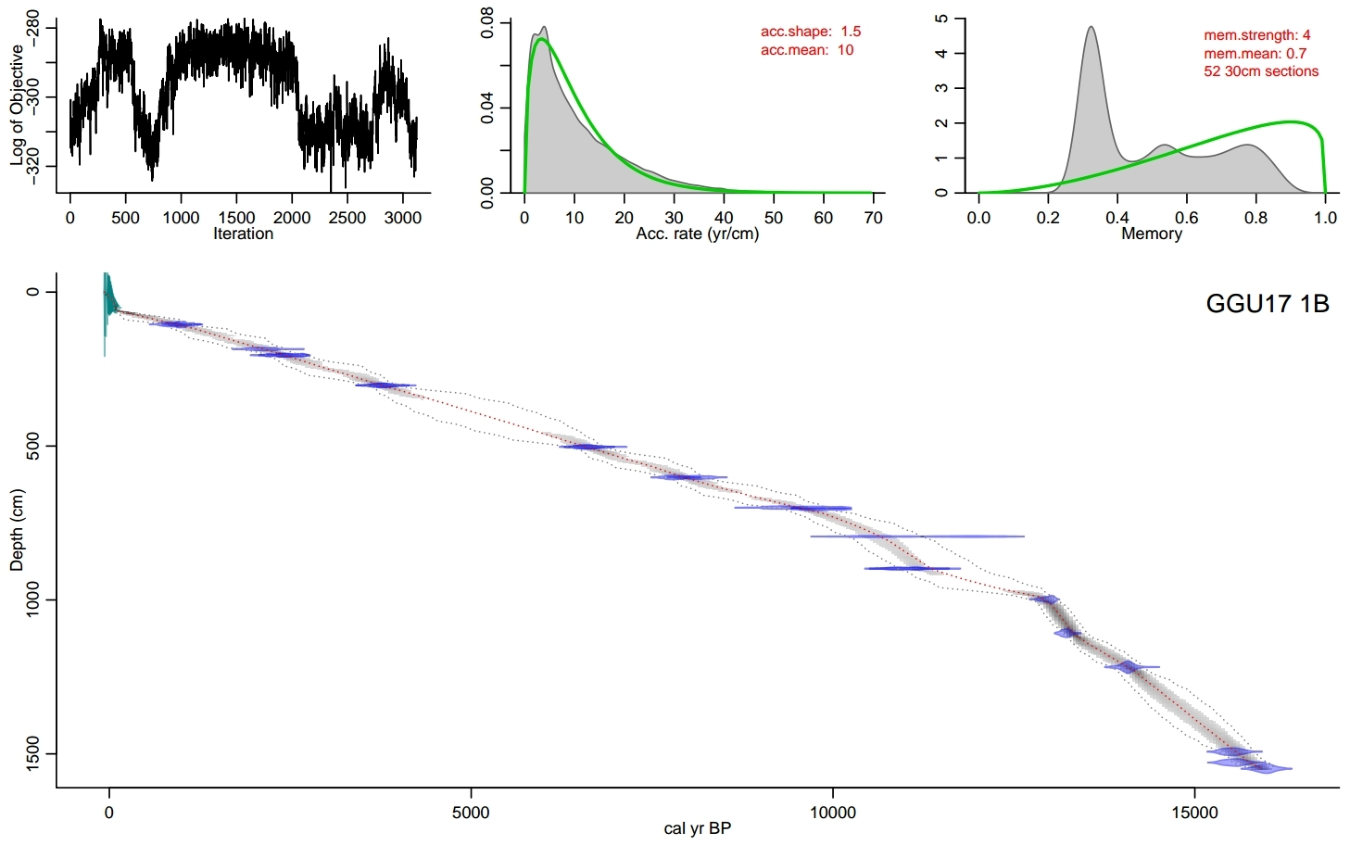
\includegraphics{Workflow_files/figure-latex/unnamed-chunk-2-1.pdf}
\caption{Bayesian age-depth model for Garba Guracha lake (3950m asl)
performed with the dates presented in ESM Table 1. More details are
found in Bittner et al {[}11{]}.}
\end{figure}

\newpage
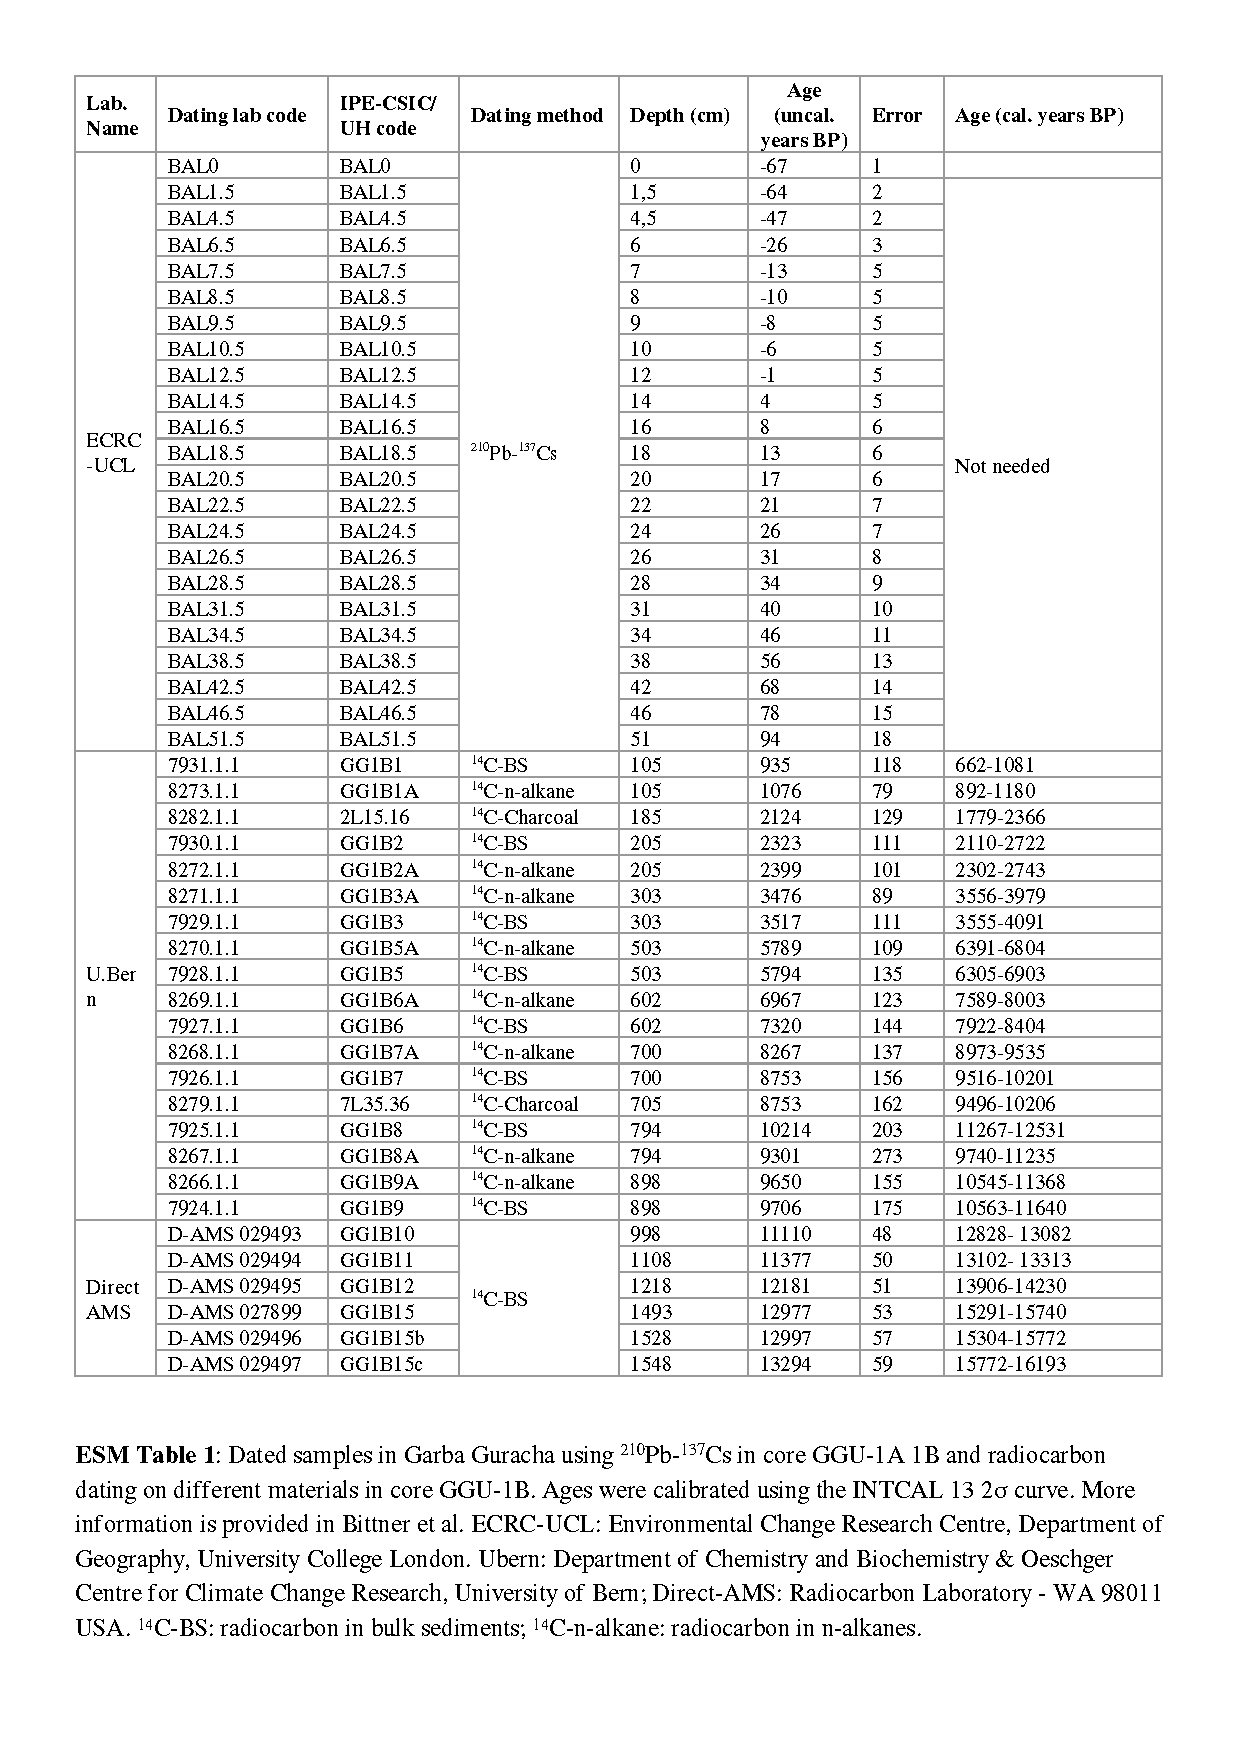
\includepdf[pages=-]{ESM_table1.pdf}

\newpage
\blandscape
\thispagestyle{empty}

\begin{figure}
\centering
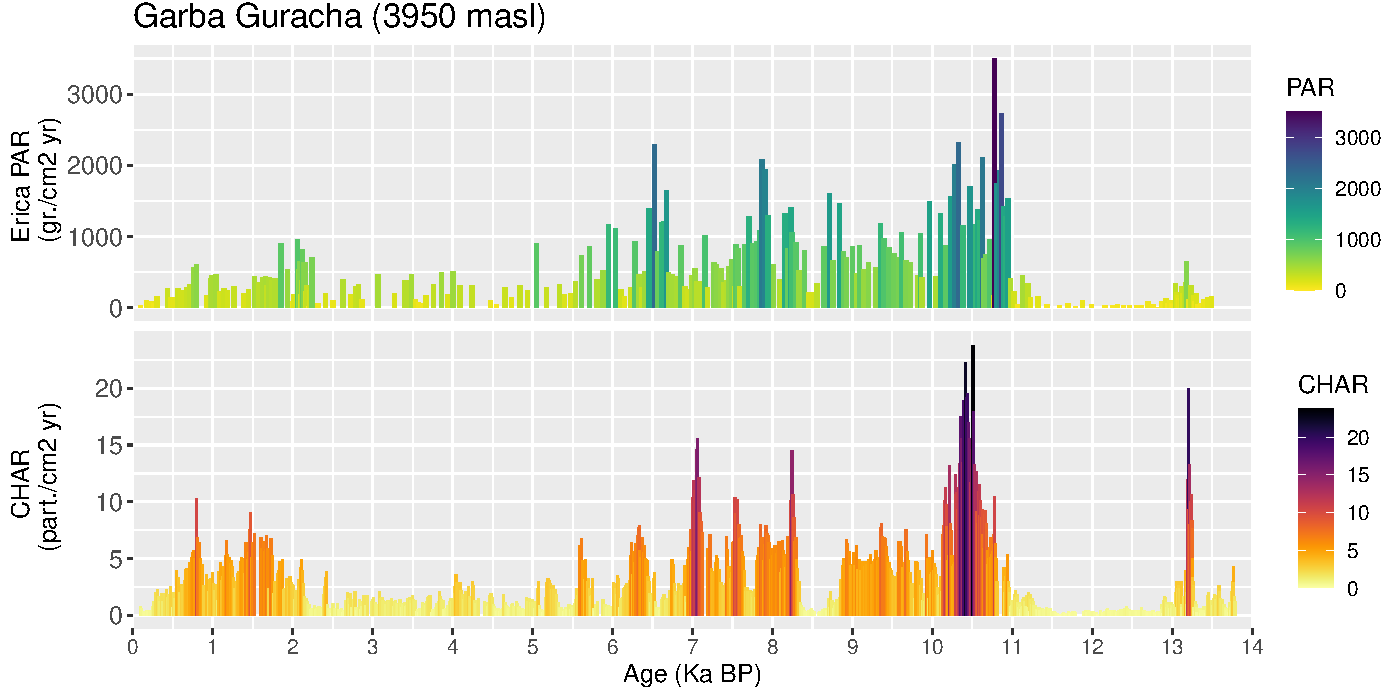
\includegraphics{Workflow_files/figure-latex/unnamed-chunk-3-1.pdf}
\caption{A) Erica PAR (grains/ cm2 year) B) CHAR (particles/ cm2 year)}
\end{figure}

\vfill
\raisebox{0.05cm}{\makebox[\linewidth]{\thepage}}
\elandscape

\hypertarget{interpolation-of-charcoal-into-regular-time-intervals}{%
\section{Interpolation of charcoal into regular time
intervals}\label{interpolation-of-charcoal-into-regular-time-intervals}}

To facilitate further analyses we interpolated the charcoal record into
100 years time-intervals. We modeled charcoal as a function of age with
\emph{loess}, by identifying the complexity value (parameter that
controls the degree of smoothing) that maximized the correlation between
observed and predicted charcoal values. We implemented the maximization
algorithm within the function \emph{interpolateDatasets}, which requires
identifying the time span defining regular time intervals over which to
interpolate the model result.

\small

\begin{Shaded}
\begin{Highlighting}[]
\CommentTok{\#requires time to find optimum span value}
\NormalTok{char.interpolated }\OtherTok{\textless{}{-}} \FunctionTok{interpolateDatasets}\NormalTok{(}
  \AttributeTok{datasets.list =} \FunctionTok{list}\NormalTok{(}\AttributeTok{char =}\NormalTok{ char), }
  \AttributeTok{age.column.name =} \StringTok{"age"}\NormalTok{, }
  \AttributeTok{interpolation.time.step =} \FloatTok{0.01} \CommentTok{\#ka}
\NormalTok{  )}
\end{Highlighting}
\end{Shaded}

\normalsize

The interpolation of charcoal into 100 years time-intervals only
generated 248 new samples. To improve the quality of the interpolation,
we replaced the interpolated values with the observed ones where
possible, as shown below.

\small

\begin{Shaded}
\begin{Highlighting}[]
\CommentTok{\#matching decimal positions in ages}
\NormalTok{char.interpolated}\SpecialCharTok{$}\NormalTok{age }\OtherTok{\textless{}{-}} \FunctionTok{round}\NormalTok{(}
\NormalTok{  char.interpolated}\SpecialCharTok{$}\NormalTok{age, }
  \DecValTok{2}
\NormalTok{  )}

\NormalTok{char}\SpecialCharTok{$}\NormalTok{age }\OtherTok{\textless{}{-}} \FunctionTok{round}\NormalTok{(}
\NormalTok{  char}\SpecialCharTok{$}\NormalTok{age, }
  \DecValTok{2}
\NormalTok{  )}

\CommentTok{\#for every age in char.interpolated}
\ControlFlowTok{for}\NormalTok{(i }\ControlFlowTok{in}\NormalTok{ char.interpolated}\SpecialCharTok{$}\NormalTok{age)\{}
  
  \CommentTok{\#getting observed value for the given age}
\NormalTok{  observed.i }\OtherTok{\textless{}{-}}\NormalTok{ char[char}\SpecialCharTok{$}\NormalTok{age }\SpecialCharTok{==}\NormalTok{ i,}\StringTok{"charcoal.acc.rate"}\NormalTok{]}
  
  \CommentTok{\#if observed.i is not empty}
  \ControlFlowTok{if}\NormalTok{(}\FunctionTok{length}\NormalTok{(observed.i) }\SpecialCharTok{\textgreater{}} \DecValTok{0}\NormalTok{)\{}
    
    \CommentTok{\#replacing interpolated by observed}
\NormalTok{    char.interpolated[}
\NormalTok{      char.interpolated}\SpecialCharTok{$}\NormalTok{age }\SpecialCharTok{==}\NormalTok{ i, }
      \StringTok{"charcoal.acc.rate"}
\NormalTok{      ] }\OtherTok{\textless{}{-}} \FunctionTok{max}\NormalTok{(observed.i) }\CommentTok{\#if two or more observed values with same age}
    
\NormalTok{  \}}
\NormalTok{\}}
\end{Highlighting}
\end{Shaded}

\normalsize

\textbf{Figure 4} shows the comparison between observed and interpolated
charcoal time-series.

\begin{figure}
\centering
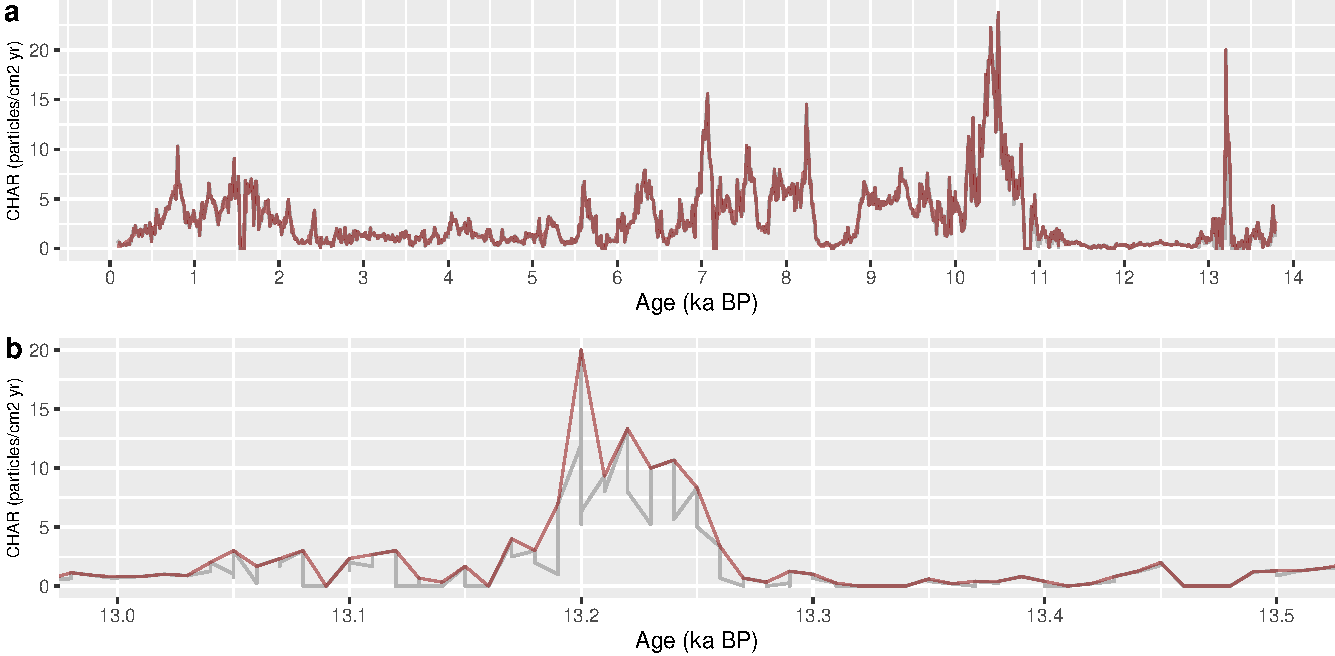
\includegraphics{Workflow_files/figure-latex/unnamed-chunk-6-1.pdf}
\caption{Comparison of observed (grey) and interpolated (red) charcoal
time series. a) Complete time series, b) Zoom on a a particular time
period where the interpolation partially decouples from real data}
\end{figure}

\#Generalised Least Squares\#

GLS provides robust estimates of regression parameters even when model
residuals are heteroscedastic {[}21{]}, a common problem of linear
models fitted on time series data. We used the R packages \emph{gls}
function of the \textbf{nlme} package {[}6{]} to fit three different
sets of models, one assessing the relationship between synchronous
values of charcoal and Erica PAR, and two others assessing time-delayed
relationships between charcoal and Erica, and viceversa.

\hypertarget{synchronous-model-concurrent-effect-of-charcoal-accumulation-rate-on-erica-abundance}{%
\subsection{Synchronous model: concurrent effect of charcoal
accumulation rate on Erica
abundance}\label{synchronous-model-concurrent-effect-of-charcoal-accumulation-rate-on-erica-abundance}}

The code below shows the procedure used to fit the synchronous model
(\textbf{Equation 1}), where Erica abundance was used as response
variable, and charcoal accumulation rate (interpolated to regular time)
as predictor. Intercept was left free, under the assumption that under
zero fire, Erica abundances would likely be higher than zero.

\textbf{Equation 1}: \[CHAR = \alpha + \beta PAR + \epsilon\]

Where:

\begin{itemize}
\tightlist
\item
  \(\alpha\) represents the intercept.
\item
  \(\beta\) is the coefficient estimate.
\item
  \(\epsilon\) is the error term.
\end{itemize}

\small

\begin{Shaded}
\begin{Highlighting}[]
\CommentTok{\#fitting GLS model}
\NormalTok{erica.char.gls }\OtherTok{\textless{}{-}} \FunctionTok{gls}\NormalTok{(}
\NormalTok{  ericaceae.par }\SpecialCharTok{\textasciitilde{}}\NormalTok{ charcoal.acc.rate,}
  \AttributeTok{data =}\NormalTok{ erica.char}
\NormalTok{  )}

\CommentTok{\#R2 (gls doesn\textquotesingle{}t provide R2)}
\NormalTok{erica.char.gls.R2 }\OtherTok{\textless{}{-}} \FunctionTok{cor}\NormalTok{(}
\NormalTok{  erica.char}\SpecialCharTok{$}\NormalTok{ericaceae.par,}
  \FunctionTok{predict}\NormalTok{(erica.char.gls)}
\NormalTok{  )}\SpecialCharTok{\^{}}\DecValTok{2}
\end{Highlighting}
\end{Shaded}

\normalsize

The model showed a R-squared (\emph{gls} does not compute R-squared) of
0.143. \textbf{Figure 4} shows the data and the fitted model.

\begin{figure}
\centering
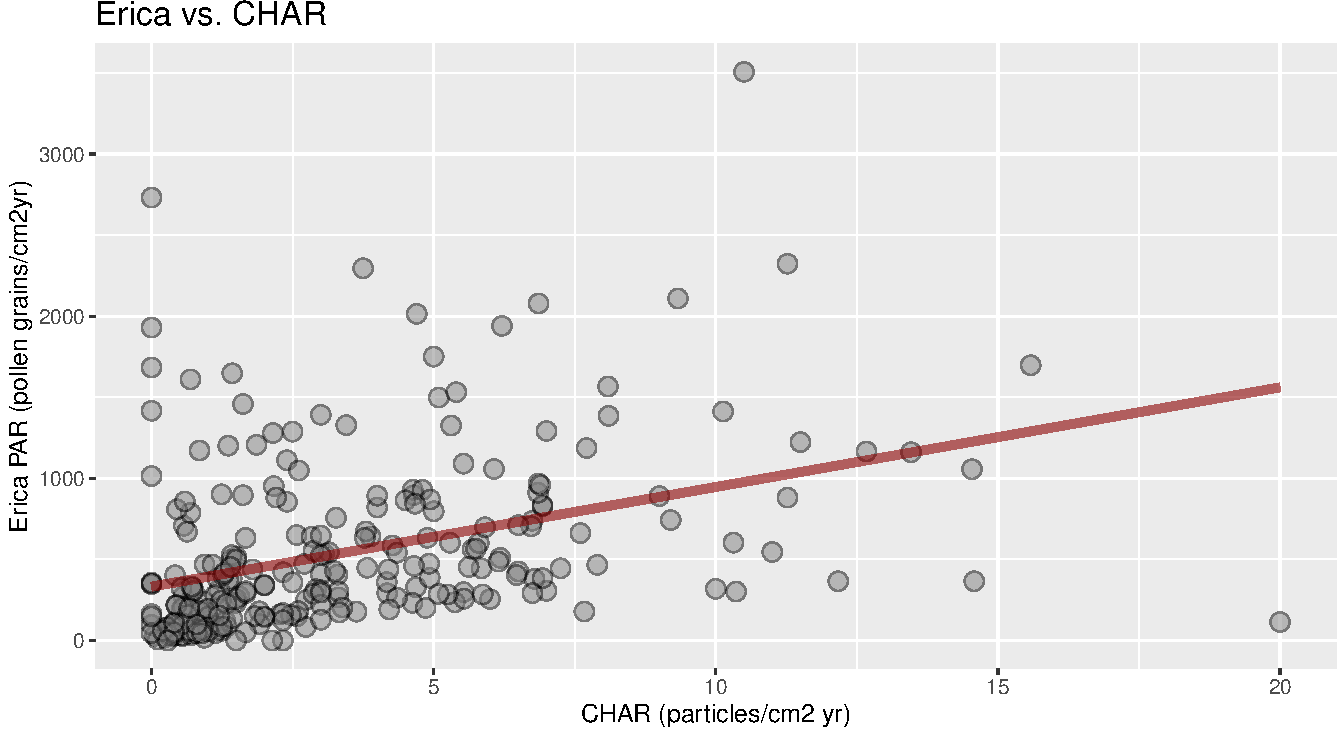
\includegraphics{Workflow_files/figure-latex/unnamed-chunk-9-1.pdf}
\caption{Erica abundances paired with synchronous samples of charcoal
accumulation rate. Straight line shows the fit of the GLS model shown
above.}
\end{figure}

\hypertarget{generating-time-delayed-lagged-data}{%
\subsubsection{Generating time-delayed (lagged)
data}\label{generating-time-delayed-lagged-data}}

The analysis described in the next section requires the data to be
expressed in time-lags, which involves aligning the samples of a given
response variable with antecedent values of a given predictor or
predictors. In our data, if we consider first Erica abundances (PAR) to
be the response variable, and interpolated charcoal accumulation rates
(CHAR) to be the predictor, for a lag of 10 years, the first PAR sample,
with age 0.23 ka BP, has to be paired with the antecedent CHAR sample,
with age 0.24 ka BP. The process is repeated for every sample and every
lag, in our case up to 100 lags (1000 years) are considered.

For this study we generate two time-lagged datasets, one were Erica
samples are paired with antecedent charcoal samples (named
\emph{lag.data.backward} in the code below), and one were charcoal
samples are paired with antecedent Erica samples (named
\emph{lag.data.forward} in the code). We selected \emph{backward} and
\emph{forward} as names because we consider \emph{Erica} samples as
reference. Therefore, the backward dataset is to assess the effect of
``past'' charcoal values on Erica, while the forward dataset is to
assess the effect of Erica on ``future'' charcoal values.

The code below uses the custom functions \textbf{backwardsLags} and
\textbf{forwardLags} to generate the datasets.

\small

\begin{Shaded}
\begin{Highlighting}[]
\CommentTok{\#100 lags}
\NormalTok{lags}\OtherTok{\textless{}{-}}\DecValTok{1}\SpecialCharTok{:}\DecValTok{101}

\CommentTok{\#forward dataset}
\NormalTok{lag.data.forward }\OtherTok{\textless{}{-}} \FunctionTok{forwardLags}\NormalTok{(}
  \AttributeTok{lags =}\NormalTok{ lags,}
  \AttributeTok{reference.data =}\NormalTok{ erica,}
  \AttributeTok{data.to.lag =}\NormalTok{ char.interpolated}
\NormalTok{  )}

\CommentTok{\#backward dataset}
\NormalTok{lag.data.backward }\OtherTok{\textless{}{-}} \FunctionTok{backwardLags}\NormalTok{(}
  \AttributeTok{lags =}\NormalTok{ lags, }
  \AttributeTok{reference.data =}\NormalTok{ erica, }
  \AttributeTok{data.to.lag =}\NormalTok{ char.interpolated}
\NormalTok{  )}
\end{Highlighting}
\end{Shaded}

\normalsize

\textbf{Figure 5} shows both datasets for lags 1 (10 years), 25 (250
years), 50 (500 years), 75 (750 years), and 100 (1000 years). It also
shows an advance of the models that will be fitted in the following
section.

\begin{figure}
\centering
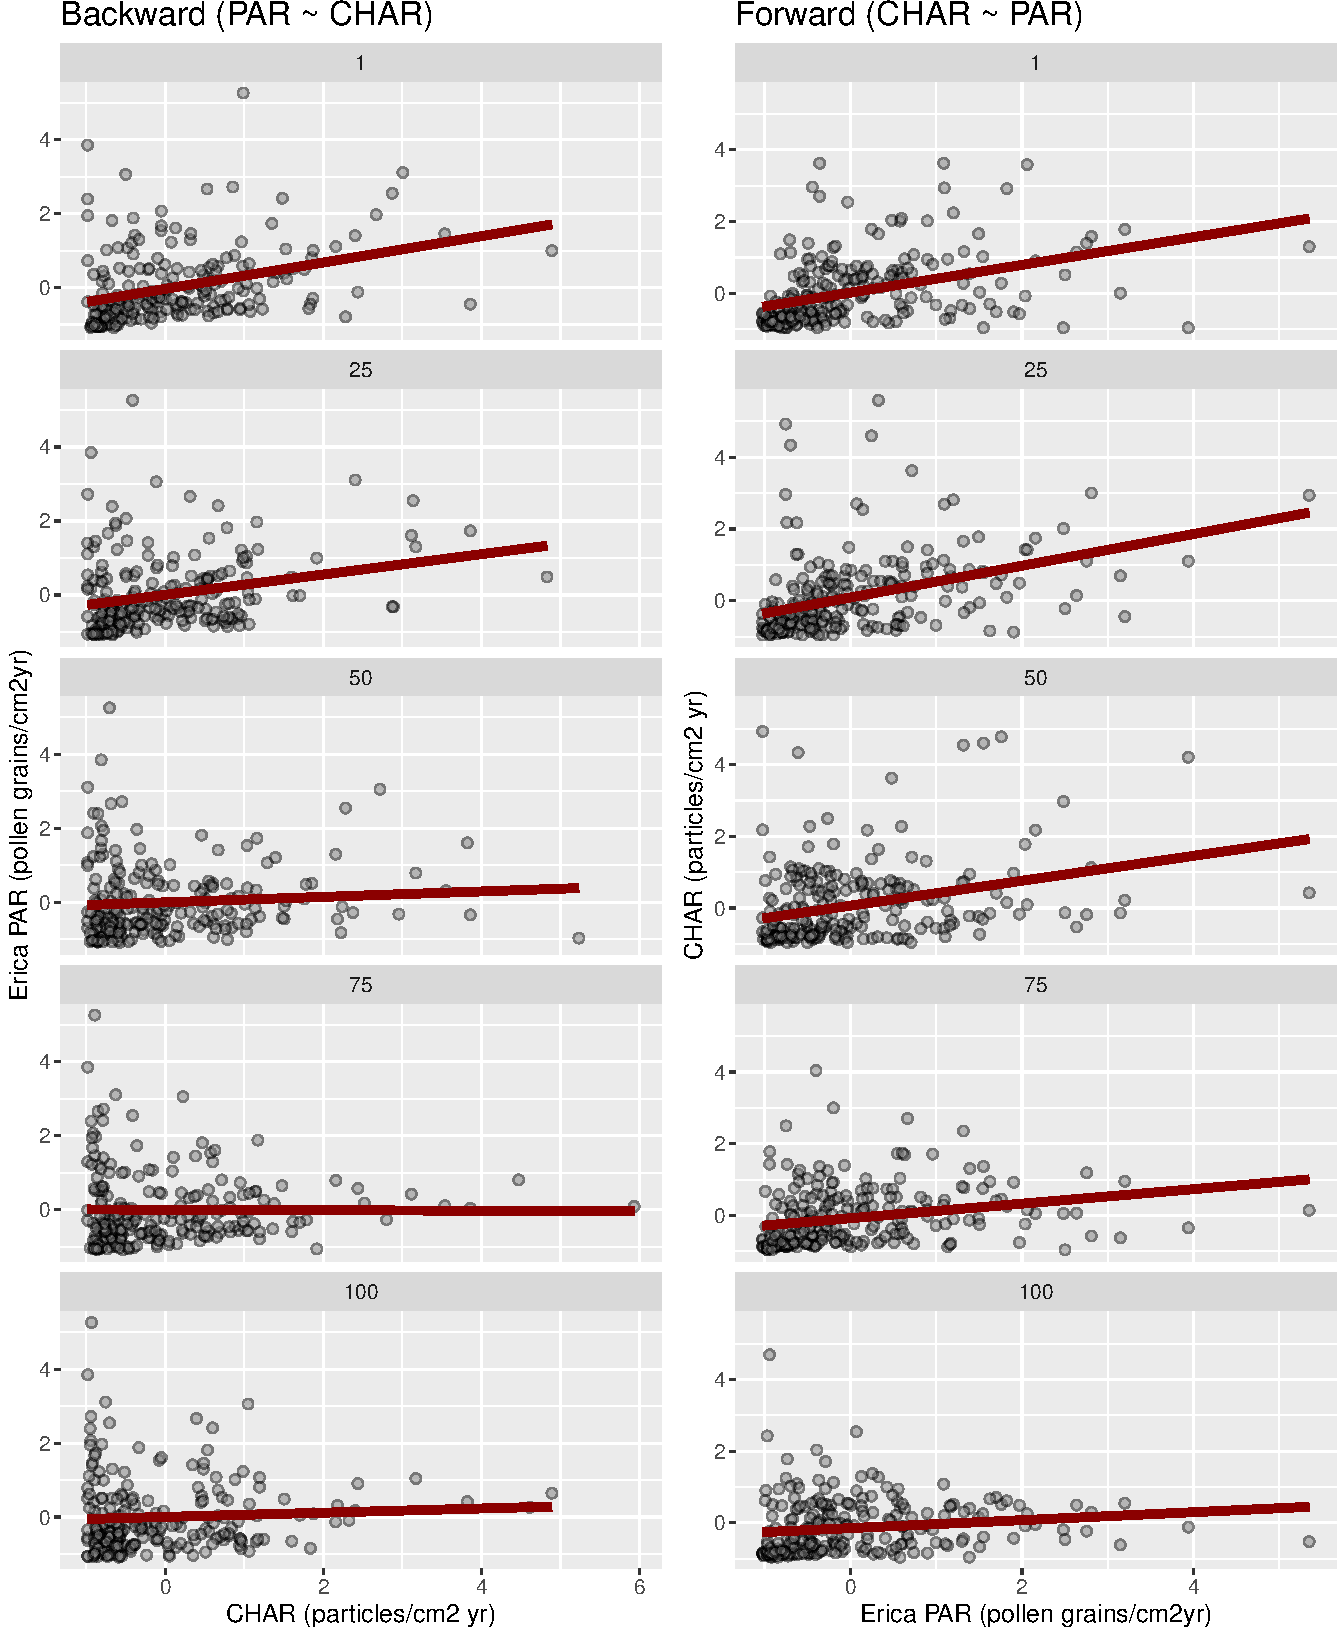
\includegraphics{Workflow_files/figure-latex/unnamed-chunk-11-1.pdf}
\caption{Lags 1, 25, 50, 75, and 100 of the backward and forward
datasets. Lag number can be found withing the grey strips. They have to
be multiplied by 10 to convert lags into years. Lines represent linear
models equivalent to those fitted in the following section.}
\end{figure}

\hypertarget{asynchronous-models-time-delayed-links-between-erica-abundance-and-charcoal-accumulation-rate}{%
\subsection{Asynchronous models: time-delayed links between Erica
abundance and charcoal accumulation
rate}\label{asynchronous-models-time-delayed-links-between-erica-abundance-and-charcoal-accumulation-rate}}

We aim to answer the questions: 1) Does Erica abundance have an effect
on subsequent charcoal accumulation rates? 2) Are there time-delayed
effects of charcoal accumulation rates on Erica abundances?;

To answer these questions we fitted two sets of \emph{asynchronous}
models described in Equations 2 and 3.

\textbf{Equation 2}:
\[CHAR_{t} = \alpha + \beta PAR_{t+lag} + \epsilon\]

\textbf{Equation 3}:
\[PAR_{t} = \alpha + \beta CHAR_{t+lag} + \epsilon\]

Where:

\begin{itemize}
\tightlist
\item
  \(t\) is the age of the given response sample.
\item
  \(lag\), with values between 10 and 1000 (in 10 years time-steps),
  represents the time-span in between the response samples and the
  antecedent samples of the given predictor.
\end{itemize}

Equations 2 and 3 were fitted once per lag on standardized data with
generalised least squares (GLS) by using the gls function of the R
package nlme {[}31{]}. R-squared and standardized coefficient estimates
with their respective confidence intervals were used to assess goodness
of fit. 100 null models on permutated response variables were fitted for
each equation to assess statistical significance.

We fitted the models through the custom function \emph{modelLagData},
that requires a formula, and a lagged dataset. The function
automatically fits one GLS model per lag, and stores R-squared values
and standardized coefficient estimates.

\small

\begin{Shaded}
\begin{Highlighting}[]
\CommentTok{\#fitting a GLS model per lag on backward datasets}
\NormalTok{backward.results }\OtherTok{\textless{}{-}} \FunctionTok{modelLagData}\NormalTok{(}
  \AttributeTok{model.formula =} \StringTok{"ericaceae.par \textasciitilde{} charcoal.acc.rate"}\NormalTok{, }
  \AttributeTok{lagged.data =}\NormalTok{ lag.data.backward}
\NormalTok{  )}

\CommentTok{\#for the forward dataset}
\NormalTok{forward.results }\OtherTok{\textless{}{-}} \FunctionTok{modelLagData}\NormalTok{(}
  \AttributeTok{model.formula =} \StringTok{"charcoal.acc.rate \textasciitilde{} ericaceae.par"}\NormalTok{, }
  \AttributeTok{lagged.data =}\NormalTok{ lag.data.forward}
\NormalTok{  )}
\end{Highlighting}
\end{Shaded}

\normalsize

\newpage

To test the deviation of coefficient estimates and R-squared from random
results we fitted each model 1000 times on permuted values of the
response. The quantiles 0.05 and 0.95 of the resulting coefficient
estimates and R-squared values were used as reference limits to
differentiate random from non-random results. This operation was
performed through the custom function \emph{modelRandomLagData}, which
takes a lagged dataset, a formula, and a number of iterations, and fits
as many GLS models as iterations indicated, with the particularity that
on each model the response is permutated. Aggregated R-squared values
and standardized coefficient estimates of these models provide a robust
null model to test the significance of our findings.

\small

\begin{Shaded}
\begin{Highlighting}[]
\NormalTok{backward.results.random }\OtherTok{\textless{}{-}} \FunctionTok{modelRandomLagData}\NormalTok{(}
  \AttributeTok{lagged.data =}\NormalTok{ lag.data.backward, }
  \AttributeTok{model.formula =} \StringTok{"ericaceae.par \textasciitilde{} charcoal.acc.rate"}\NormalTok{, }
  \AttributeTok{iterations =} \DecValTok{1000}
\NormalTok{  )}

\NormalTok{forward.results.random }\OtherTok{\textless{}{-}} \FunctionTok{modelRandomLagData}\NormalTok{(}
  \AttributeTok{lagged.data =}\NormalTok{ lag.data.forward, }
  \AttributeTok{model.formula =} \StringTok{"charcoal.acc.rate \textasciitilde{} ericaceae.par"}\NormalTok{, }
  \AttributeTok{iterations =} \DecValTok{1000}
\NormalTok{  )}
\end{Highlighting}
\end{Shaded}

\normalsize

Coefficient estimates with their standard errors and R-squared values
were extracted from each model and plotted against lagged age to
facilitate the interpretation of the results. \textbf{Figure 7} shows
the results of the fitted models.

\begin{figure}
\centering
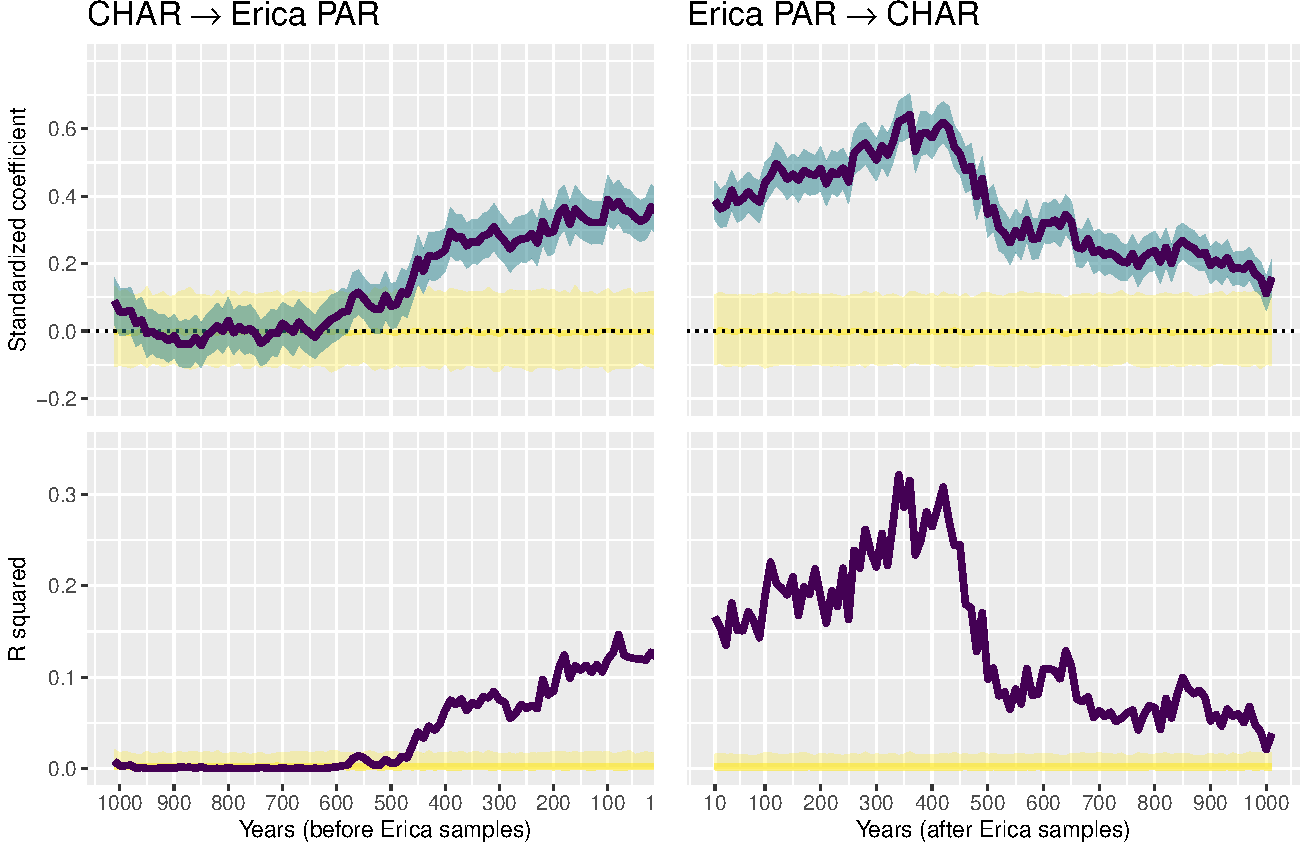
\includegraphics{Workflow_files/figure-latex/unnamed-chunk-14-1.pdf}
\caption{Results of the time-lagged models. Left panel represents models
fitted with Equation 1, that is, the influence of antecedent values of
CHAR on the pollen abundance of Erica (PAR) across time-lags up to 1000
years. The right panel represents the influence of antecedent values of
Erica PAR on CHAR over the same time-lags. Yellow strips represent
standardized coefficients and R-squared values for the null model. Data
not intersecting yellow strips is interpreted as statistically
significant.}
\end{figure}

\newpage

\hypertarget{bibliography}{%
\section{Bibliography}\label{bibliography}}

{[}1{]} Urbanek, S. png: Read and write PNG images
\url{https://cran.r-project.org/web/packages/png/index.html}. 2013.

{[}2{]} R Core Team. R: A Language and Environment for Statistical
Computing. Vienna, Austria: R Foundation for Statistical Computing.
\url{https://www.R-project.org/}. 2018.

{[}3{]} Wickham, H. Ggplot2: Elegant Graphics for Data Analysis.
Springer-Verlag New York. \url{http://ggplot2.org}. 2016.

{[}4{]} Wickham, H. and Lionel, H. Tidyr: Easily Tidy Data with
'Spread()' and 'Gather()' Functions.
\url{https://CRAN.R-project.org/package=tidyr.2018}.

{[}5{]} Garnier, Simon. Viridis: Default Color Maps from 'Matplotlib'.
\url{https://CRAN.R-project.org/package=viridis}. 2018.

{[}6{]} Pinheiro J, et al.~nlme: Linear and Nonlinear Mixed Effects
Models. R package version 3.1-137,
\url{https://CRAN.R-project.org/package=nlme}. 2018.

{[}7{]} Wilke, C. Cowplot: Streamlined Plot Theme and Plot Annotations
for 'Ggplot2'. \url{https://CRAN.R-project.org/package=cowplot.2019}.

{[}8{]} Xie, Y. FormatR: Format R Code Automatically.
\url{https://CRAN.R-project.org/package=formatR.2017}.

{[}9{]} Xie, Y.Knitr: A General-Purpose Package for Dynamic Report
Generation in R. \url{https://yihui.name/knitr/}. 2018.

{[}10{]} Tiercelin, J.J. et al., ``High-resolution sedimentary record of
the last deglaciation from a high-altitude lake in Ethiopia,''
Quaternary Science Reviews, vol.~27, no. 5, pp.~449--467, Mar.~2008.

{[}11{]} Clark, J.S. and Royall,P.D. Local and regional sediment
charcoal evidence for fire regimes in presettlement north-eastern North
America. Journal of Ecology, vol.~84, pp.~365--382, 1996.

{[}12{]} Higuera, P.E., et al.~Understanding the origin and analysis of
sediment-charcoal records with a simulation model. Quaternary Science
Reviews, vol.~26, no. 13--14, pp.~1790--1809, 2007.

{[}13{]} Adolf, C. et al., The sedimentary and remote-sensing reflection
of biomass burning in Europe. Global Ecol Biogeogr, vol.~27, no. 2,
pp.~199--212, 2018.

{[}14{]} Oris, F. et al., `Charcoal dispersion and deposition in boreal
lakes from 3 years of monitoring: Differences between local and regional
fires', Geophysical Research Letters, vol.~41, no.2, p.~6743-6752. doi:
10.1002/2014GL060984, Aug.~2014.

{[}15{]} Davis, M.B. On the theory of pollen analysis. American Journal
of Science, vol.~261, no. 10, pp 897--912. 1963.

{[}16{]} Davis, M.B. Redepostion of pollen grains in lake sediments.
Limnology and Oceanography, vol.~18, no. 1, pp.~44--52, Jan.~1973.

{[}17{]} Schüler, et al., ``Relationship between vegetation and modern
pollen-rain along an elevational gradient on Kilimanjaro, Tanzania,''
The Holocene, vol.~24, no. 6, pp 702-713. 2014.

{[}18{]} Bonnefille, R. and Riollet,G. The Kashiru Pollen Sequence
(Burundi) Palaeoclimatic Implications for the last 40,000 yr B.P. in
Tropical Africa. Quaternary Research, vol.~30, pp.~19--35, 1988.

{[}19{]} Moore, P.D., Collinson, M., Webb, J.A. Pollen Analysis, New
Edition of 2 Revised Edition. Wiley-Blackwell. 216 pp.~1994.

{[}20{]} Stockmarr, J., 1973. Determination of spore concentration with
an electronic particle counter. Danm.geol.Unders. Arbog 1972, 87--89.

{[}21{]} Blaauw, M. and Christen,J.A. Flexible paleoclimate age-depth
models using an autoregressive gamma process. Bayesian Analysis vol.~6,
no. 3, pp.~457--474, 2011.

{[}22{]} Aitken,A.C. ``IV.---On Least Squares and Linear Combination of
Observations,'' Proceedings of the Royal Society of Edinburgh, vol.~55,
pp.~42--48, 1936.

\end{document}
